\question 对一个无噪声的4kHz信道进行采样,可达到的最大数据传输速率是( )
\par\twoch{4kbit/s}{8kbit/s}{1kbit/s}{\textcolor{red}{无限大}}
\begin{solution}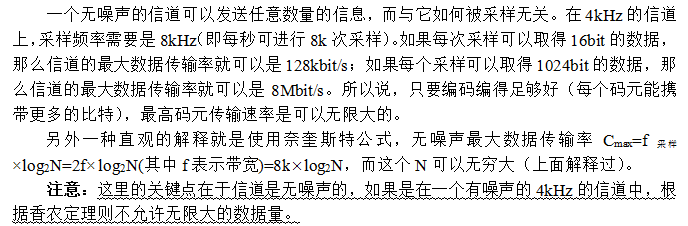
\includegraphics[width=3.70833in,height=1.21875in]{computerassets/B0AE585B95CFFFFD9D175FCB4B196857.png}
\end{solution}
\question 一个信道每1/8s采样一次,传输信号共有16种变化状态,则最大数据传输速率是(
)
\par\twoch{16bit/s}{\textcolor{red}{32bit/s}}{48bit/s}{64bit/s}
\begin{solution}信道每1/8s采样一次,说明采样频率为8Hz。由采样定理可知,采样频率必须大于或等于最大频率的两倍。也就是说,此信道的最高频率为4Hz,既然是要求最大数据传输速率,不妨设最小频率为0Hz,那么就可以求出最大带宽=最高频率-最低频率=4Hz。于是就可以使用奈奎斯特定理来计算,即最大数据传输速率=2×4×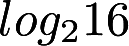
\includegraphics[width=0.46875in,height=0.15625in]{texmath/8d88685Cdpi7B3507Dlog_216}=32bit/s。当然,此题也可以直接使用公式:Cmax=f采样×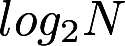
\includegraphics[width=0.45833in,height=0.14583in]{texmath/b7c31d5Cdpi7B3507Dlog_2N}=8×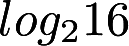
\includegraphics[width=0.46875in,height=0.15625in]{texmath/8d88685Cdpi7B3507Dlog_216}=32bit/s。
\end{solution}
\question 要在带宽为4kHz的信道上用2s发送80kbit的数据块,按照香农公式,信道的信噪比最小为(
)dB
\par\twoch{1024}{1023}{\textcolor{red}{31}}{30}
\begin{solution}其实这道题目就是变相地给出了最大传输速率=80kbit/2s=40kbit/s。那么使用香农公式可以得到:40kbit/s=4kHz×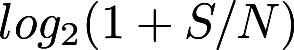
\includegraphics[width=1.05208in,height=0.18750in]{texmath/07e0fd5Cdpi7B3507Dlog_22812BS2FN29},解得S/N=2\^{}10-1=1023,然后将其转换为分贝,即10lg(S/N)。而30小于10lg(S/N)小于31,故信道的信噪比最小为31dB,才能达到所需的最大传输速率。
\end{solution}
\question 假设一个无噪声的信道,带宽是6MHz,并且采用了4级数字信号,那么它每秒可发送的数据量为(
)
\par\twoch{6Mbit}{12Mbit}{\textcolor{red}{24Mbit}}{48Mbit}
\begin{solution}根据奈奎斯特定理,可以对信道每秒采样12M次。因为是4级数字信号,每次采样可获得2bit的数据,所以总共的数据传输率是24Mbit/s,即每秒发送了24Mbit的数据。
提醒:4级数字信号指什么?这个无需知道,在考研中,只需记住一点,看到这种条件,直接log2即可,得到有用的信息。
\end{solution}
